\begin{savequote}[45mm]
\ascii{Any fool can write code that a computer can understand. Good programmers write code that humans can understand.}
\qauthor{\ascii{- Martin Flower}}
\end{savequote}

\chapter{介绍} 
\label{ch:introduction}

\begin{content}

\tf{}是一个使用\emph{数据流图}\ascii{(Dataflow Graph)}表达数值计算的开源软件库。它使用\emph{节点}表示抽象的数学计算,并使用\ascii{OP}表达计算的逻辑;而\emph{边}表示节点间传递的数据流,并使用\ascii{Tensor}表达数据的表示。\upcite{tf-white-paper}。数据流图是一种\emph{有向无环图}\ascii{(DAG)},当图中的\ascii{OP}按照特定的拓扑排序依次被执行时,\ascii{Tensor}在图中流动形成数据流,\tf{}因此而得名。

在分布式运行时,数据流图的被分裂为多个子图,并被有效地部署到集群中的多个机器上并发执行。在一个机器内,注册的子图被二次分裂为更小的子图,它们被部署在\emph{本地设备集}上并发执行。\tf{}支持多种异构设备的分布式计算,包括\ascii{CPU, GPU, ASIC}。\tf{}跨平台的卓越表现,使得它能够灵活地部署在各种计算平台上,包括台式机、服务器、移动终端。

\tf{}最初由\ascii{Google Brain}的研究员和工程师们开发出来,用于开展机器学习和深度神经网络的研究,包括语言识别、计算机视觉、自然语言理解、机器人、信息检索。但是,\tf{}系统架构的通用性和灵活性,使其广泛地用于其他科学领域的数值计算。

\end{content}

\section{前世今生}

\begin{content}

\ascii{Google Brain}项目始于\ascii{2011}年,用于研究超大规模的深度神经网络。在项目早期阶段,\ascii{Google Brain}构建了第一代分布式深度学习框架\ascii{DistBelief},并在\ascii{Google}内部的产品中得到了大量的应用。

基于\ascii{DistBelief}的经验,\ascii{Google Brain}对深度学习训练和推理的需求,及其深度学习框架的系统行为和属性,有了更全面更深刻地理解,并于\ascii{2015.11}重磅推出第二代分布式深度学习框架\tf{}。\tf{}作为\ascii{DistBelief}的后继者,革命性地对既有系统架构做了全新设计和实现,\tf{}一经发布,便在深度学习领域一鸣惊人,在社区中形成了巨大的影响力。

\subsection{DistBelief}

\ascii{DistBelief}是一个用于训练大规模神经网络的的分布式系统,是\ascii{Google}第一代分布式机器学习框架。自\ascii{2011}年以来,在\ascii{Google}内部大量使用\ascii{DistBelief}训练大规模的神经网络,并广泛地用于机器学习和深度学习领域的研究和应用,包括非监督学习、语言表示、图像分类、目标检测、视频分类、语音识别、序列预测、行人检测、强化学习等。

\subsubsection{编程模型}

\ascii{DistBelief}的编程模型是基于\emph{层}的\ascii{DAG}图。层可以看做是一种组合多个运算操作符的复合运算符,它完成特定的计算任务。例如,全连接层完成$f({W^T}x + b)$的复合计算,包括输入与权重的矩阵乘法,随后再与偏置相加,最后在线性加权值的基础上应用激活函数,实施非线性变换。

\subsubsection{架构}

\ascii{DistBelief}使用\emph{参数服务器}\ascii{(Parameter Server, 常称为PS)}的系统架构,训练作业包括两个分离的进程:无状态的\ascii{Worker}进程,用于模型的训练;有状态的\ascii{PS}进程,用于维护模型的参数。如\refig{parameter-server}所示,在分布式训练过程中,各个\emph{模型副本}异步地从\ascii{PS}上拉取训练参数$w$,当完成一步迭代运算后,推送参数的梯度$ \Delta w $到\ascii{PS}上去,并完成参数的更新。

\begin{figure}[H]
\centering
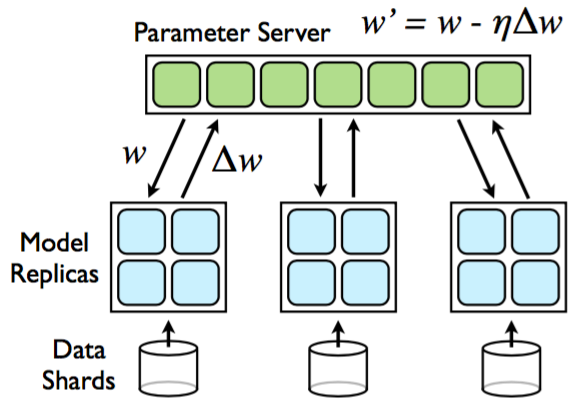
\includegraphics[width=0.5\textwidth]{figures/parameter-server.png}
\caption{DistBelief: Parameter Server架构}
 \label{fig:parameter-server}
\end{figure}

\subsubsection{缺陷}

但是,对于深度学习领域的高级用户,\ascii{DistBelief}的编程模型,及其基于\ascii{PS}的系统架构,缺乏足够的灵活性和可扩展性。

\begin{enum}
  \eitem{优化算法:添加新的优化算法,必须修改\ascii{PS}的实现;\code{get(), put()}的抽象方法,对某些优化算法并不高效。}
  \eitem{训练算法:支持非前馈的神经网络面临巨大的挑战性;例如,包含循环的\ascii{RNN},交替训练的对抗网络,及其损失函数由分离的代理完成的增强学习模型。} 
  \eitem{加速设备:\ascii{DistBelief}设计之初仅支持多核\ascii{CPU},并不支持多卡的\ascii{GPU},遗留的系统架构对支持新的计算设备缺乏良好的可扩展性。}
\end{enum}

\subsection{TensorFlow}

\ascii{DistBelief}遗留的架构和设计,不再满足深度学习与日俱增的需求变化,\ascii{Google}毅然放弃了既有的\ascii{DistBelief}实现,并决定在其基础上做全新的系统架构设计,\ascii{TensorFlow}应运而生,开创了深度学习领域的新纪元。

\subsubsection{编程模型}

\ascii{TensorFlow}使用数据流图表达计算过程和共享状态,使用节点表示抽象计算,使用边表示数据流。如\refig{tf-dataflow}所示,展示了\ascii{MNIST}手写识别应用的数据流图。在该模型中,前向子图使用了\ascii{2}层全连接网络,分别为\ascii{ReLU}层和\ascii{Softmax}层。随后,使用\ascii{SGD}的优化算法,构建了与前向子图对应的反向子图,用于计算训练参数的梯度。最后,根据参数更新法则,构造训练参数的更新子图,完成训练参数的迭代更新。

\begin{figure}[H]
\centering
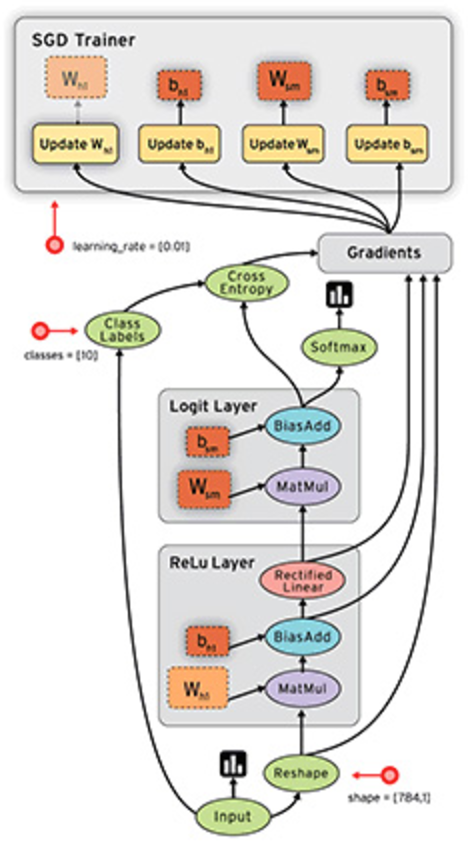
\includegraphics[width=0.4\textwidth]{figures/tf-dataflow.png}
\caption{TensorFlow: 数据流图}
 \label{fig:tf-dataflow}
\end{figure}

\subsubsection{设计原则}

\tf{}的系统架构遵循了一些基本的设计原则,用于指导\tf{}的系统实现。

\begin{enum}
  \eitem{延迟计算:图的构造与执行分离,并推迟计算图的执行过程;}
  \eitem{原子\ascii{OP}:\ascii{OP}是最小的抽象计算单元,支持构造复杂的网络模型;} 
  \eitem{抽象设备:支持\ascii{CPU, GPU, ASIC}多种异构计算设备类型;}
  \eitem{抽象任务:基于任务的\ascii{PS},对新的优化算法和网络模型具有良好的可扩展性。}  
\end{enum}

\subsubsection{优势}

相对于其他机器学习框架,\ascii{TensorFlow}具有如下方面的优势。

\begin{enum}
  \eitem{高性能:\tf{}升级至\ascii{1.0}版本性能提升显著,单机多卡(\ascii{8}卡\ascii{GPU})环境中,\ascii{Inception v3}的训练实现了\ascii{7.3}倍的加速比;在分布式多机多卡(\ascii{64}卡\ascii{GPU})环境中,\ascii{Inception v3}的训练实现了\ascii{58}倍的加速比;}
  \eitem{跨平台:支持多\ascii{CPU/GPU/ASIC}多种异构设备的运算;支持台式机,服务器,移动设备等多种计算平台;支持\ascii{Windows,Linux,MacOS}等多种操作系统;}
  \eitem{分布式:支持本地和分布式的模型训练和推理;}
  \eitem{多语言:支持\ascii{Python, C++, Java, Go}等多种程序设计语言;}  
  \eitem{通用性:支持各种复杂的网络模型的设计和实现,包括非前馈型神经网络;}
  \eitem{可扩展:支持\ascii{OP}扩展,\ascii{Kernel}扩展,\ascii{Device}扩展,通信协议的扩展;}
  \eitem{可视化:使用\ascii{TensorBoard}可视化整个训练过程,极大地降低了\tf{}的调试过程;}
  \eitem{自动微分:\tf{}自动构造反向的计算子图,完成训练参数的梯度计算;}
  \eitem{工作流:\ascii{TensorFlow}与\ascii{TensorFlow Serving}无缝集成,支持模型的训练、导入、导出、发布一站式的工作流,并自动实现模型的热更新和版本管理。}      
\end{enum}

\end{content}

\section{社区发展}

\begin{content}

\tf{}是目前炙手可热的深度学习框架。自开源以来,\tf{}社区相当活跃。在\ascii{Github}上收获了来自众多的非\ascii{Google}员工的数万次代码提交,并且每周拥有近百个\ascii{Issue}被提交。在\ascii{Stack Overflow}上也拥有上万个关于\tf{}的问题被提问和回答。在各种技术大会上,\tf{}也是一颗闪亮的明星,得到众多开发者的青睐。

\subsection{开源}

\ascii{2015.11},\ascii{Google Research}发布文章:\code{\href{https://research.googleblog.com/2015/11/tensorflow-googles-latest-machine\_9.html}{TensorFlow: Google's latest machine learning system, open sourced for everyone}},正式宣布新一代机器学习系统\ascii{TensorFlow}开源。随后,\ascii{TensorFlow}在\ascii{Github}上代码仓库短时间内获得了大量的\ascii{Star}和\ascii{Fork}。如\refig{tf-commits}所示,\ascii{TensorFlow}的社区活跃度已远远超过其他竞争对手,成为目前最为流行的深度学习框架。

\begin{figure}[H]
\centering
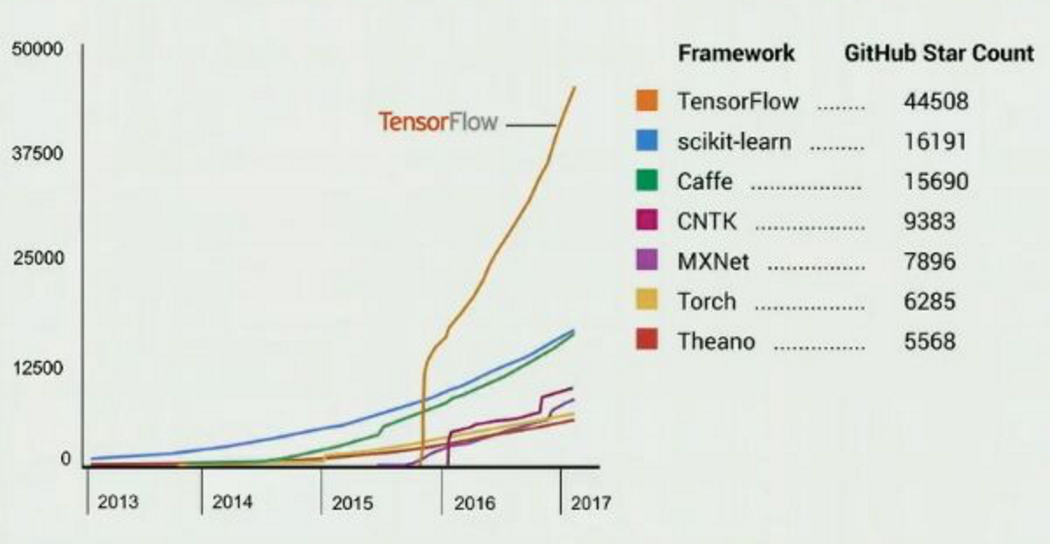
\includegraphics[width=1.0\textwidth]{figures/tf-commits.png}
\caption{TensorFlow:社区活跃度}
 \label{fig:tf-commits}
\end{figure}

毫无疑问,\ascii{TensorFlow}的开源对学术界和工业界产生了巨大的影响,它极大地降低了深度学习在各个行业中应用的难度。众多的学者、工程师、企业、组织纷纷地投入到了\ascii{TensorFlow}社区,并一起完善和改进\ascii{TensorFlow},推动其不断地向前演进和发展。

\subsection{里程碑}

\tf{}自\ascii{2015.11}开源以来,平均一个多月发布一个版本。如\refig{tf-versions}所示,展示了\tf{}几个重要特性的发布时间。

\begin{figure}[!htbp]
\centering
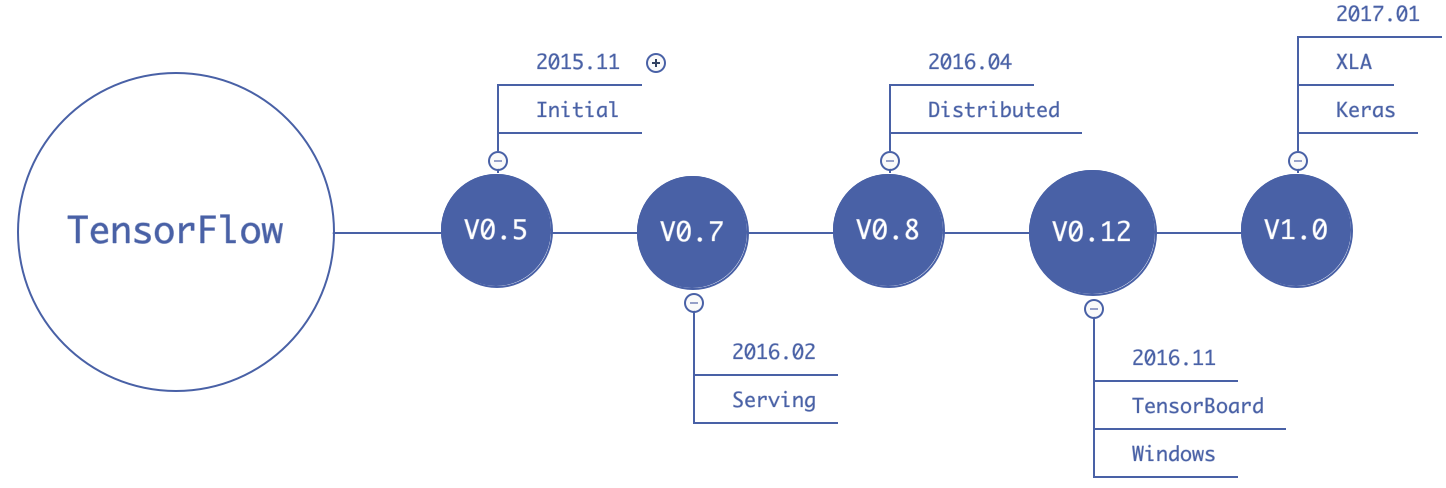
\includegraphics[width=1.0\textwidth]{figures/tf-versions.png}
\caption{TensorFlow重要里程碑}
 \label{fig:tf-versions}
\end{figure}

\subsection{工业应用}

\ascii{TensorFlow}自开源发展两年以来,在生产环境中被大量应用使用。在医疗方面,帮助医生预测皮肤癌发生的概率;在音乐、绘画领域,帮助人类更好地理解艺术;在移动端,多款移动设备搭载\ascii{TensorFlow}训练的机器学习模型,用于翻译工作。\ascii{TensorFlow}在\ascii{Google}内部应用的增长也十分迅速,多个重量级产品都有相关应用,包括:\ascii{Google Search, Google Gmail, Google Translate, Google Maps}等,如\refig{tf-google-apps}所示。

\begin{figure}[!htbp]
\centering
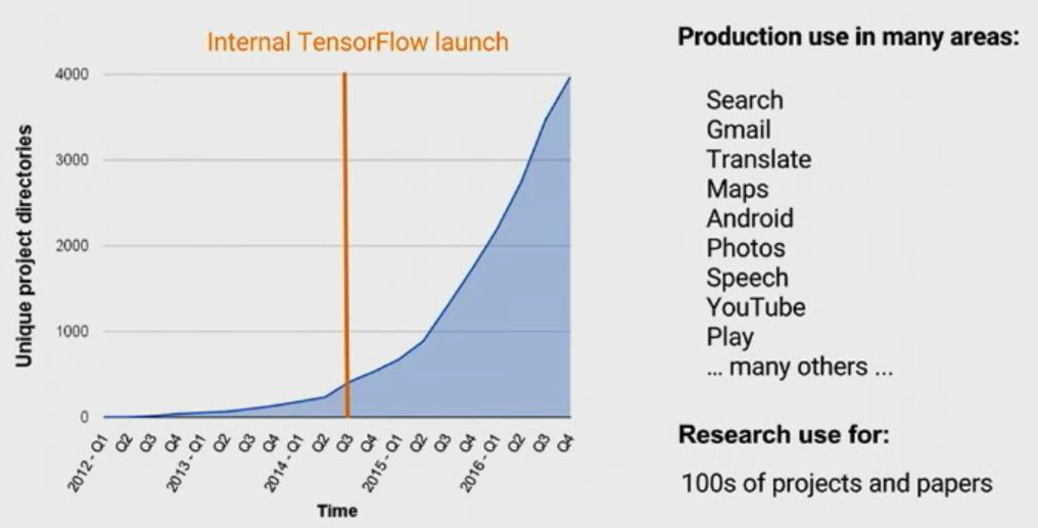
\includegraphics[width=1.0\textwidth]{figures/tf-google-apps.png}
\caption{TensorFlow:在Google内部使用情况}
 \label{fig:tf-google-apps}
\end{figure}

\end{content}